\documentclass{beamer}

\usepackage{graphics}
\usepackage{graphicx}
\usepackage{amsmath,amssymb,amsthm}
\usepackage{cancel}
%\usepackage{subeqnarray}
%\usepackage{easybmat}
%\usepackage{subfigure}



%\usepackage{HA-prosper}
%\usepackage[dvips,letterpaper]{geometry}

\def\Proba#1{\mathcal{P}\left(#1\right)}
\def\Surv{\mathcal{S}}
\def\R{\mathcal{R}}
\def\D{\mathcal{D}}
\def\C{\mathcal{C}}
\def\M{\mathcal{M}}
\def\L{\mathcal{L}}
\def\IC{\mathbb{C}}
\def\IN{\mathbb{N}}
\def\IR{\mathbb{R}}
\def\IZ{\mathbb{Z}}
\def\IK{\mathbb{K}}
\def\II{\mathbb{I}}
\def\Rzero{\mathcal{R}_0}
\newcommand{\diag}{\operatorname{diag}}
\def\tr{\textrm{tr}}
\def\det{\textrm{det}}
\def\sgn{\textrm{sgn}}
\def\imply{$\Rightarrow$}
\def\dbint{\int\!\!\!\int}
\def\dbintb{\mathop{\int\!\!\!\!\int}}
\def\tpint{\int\!\!\!\int\!\!\!\int}

\def\red{\color[rgb]{1,0,0}}

\newtheorem{proposition}{Proposition}

\setbeamertemplate{navigation symbols}{}
\setbeamertemplate{footline}
{%
\quad\insertsection\hfill p. \insertpagenumber\quad\mbox{}\vskip2pt
}

\title[Shallow water]{Shallow water\\[1.5cm] Partial differential equations}
\date{}

\begin{document}
\frame[plain]{\setcounter{page}{0}\titlepage}
%%%%%%%%%%%%%%
%%%%%%%%%%%%%%


\section{Model formulation}
\frame[plain]{\tableofcontents[current]}

\frame{\frametitle{Spatial domain}
We consider the motion of a body of water that is infinite in the $z$ direction, with or without boundary in the $x$ direction, and the vertical direction of gravity taken as the $y$ direction.
\begin{center}
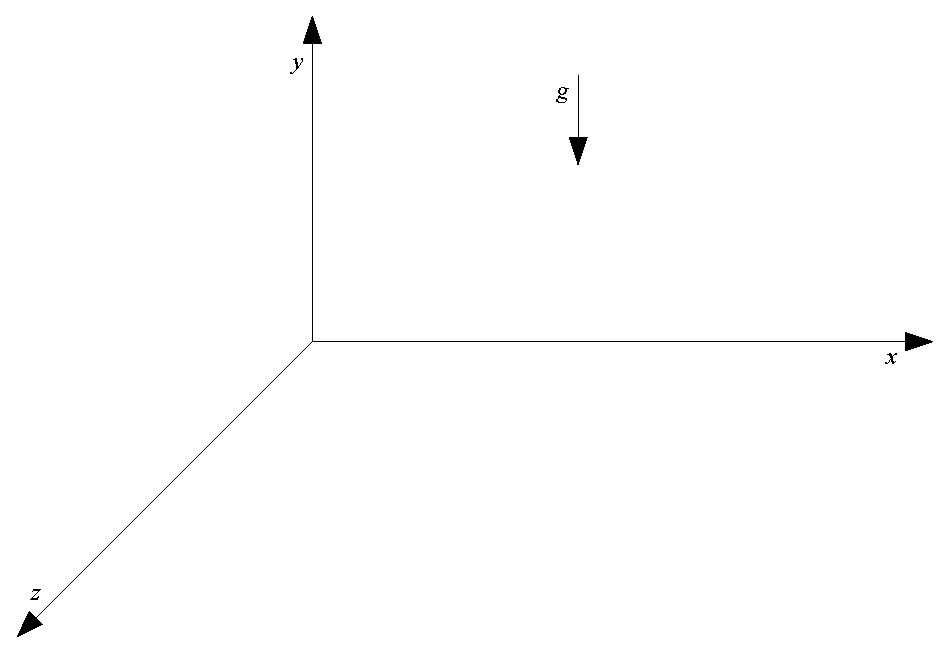
\includegraphics[width=0.7\textwidth]{xyz_domain}
\end{center}
From now on, suppose $z$ direction uniform (the same for all $z$), so ignore $z$ except for the sake of argument.
}

\frame{
\begin{itemize}
\item Water depth at rest, $H$, small compared to distance $L_0$ over which significant changes can occur in the $x$ direction.
\item Undisturbed water surface, $y=0$.
\item Moving upper free surface $y=\eta$, measured from $y=0$.
\item Sea floor $y=-H$.
\end{itemize}
\begin{center}
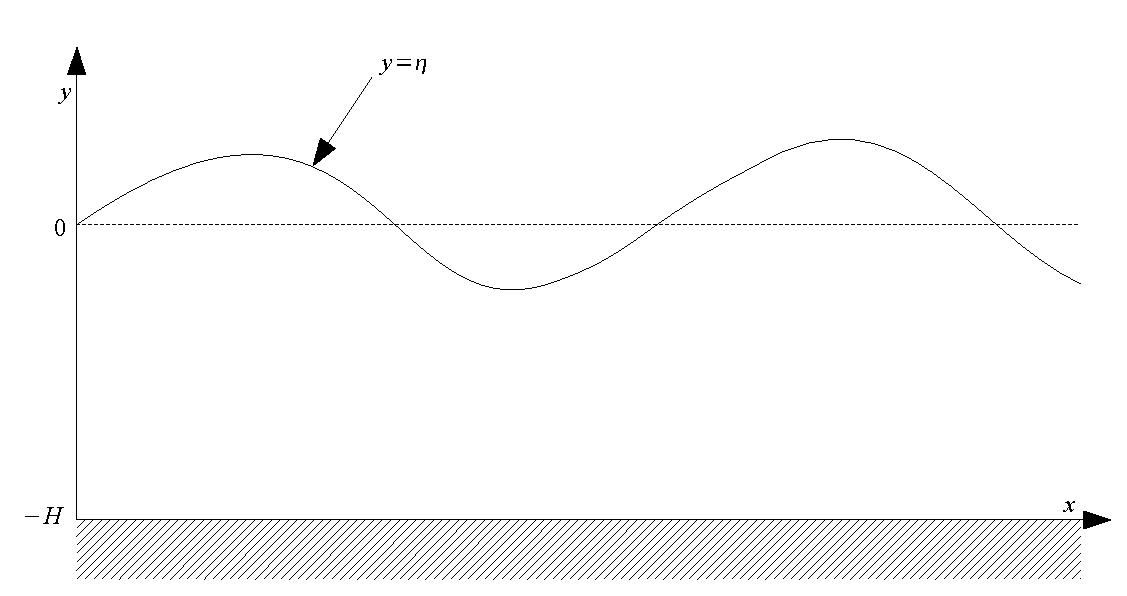
\includegraphics[width=0.7\textwidth]{xy_domain}
\end{center}
}

\frame{
\begin{itemize}
\item $u$ velocity in the $x$ direction. Assume independent of depth $y$.
\item $\rho$ mass density of water.
\item $p(x,y,t)$ pressure in fluid at point $(x,y)$ at time $t$. In water, magnitude at any $(x,y)$ is same in all directions.
\end{itemize}
Fluid motion independent of $z$, so
\begin{itemize}
\item $u=u(x,t)$
\item $\eta=\eta(x,t)$.
\end{itemize}
}


\frame{
Take a cylindrical water column, with base area $A$, between $y_1$ and $y_2>y_1$.
\begin{center}
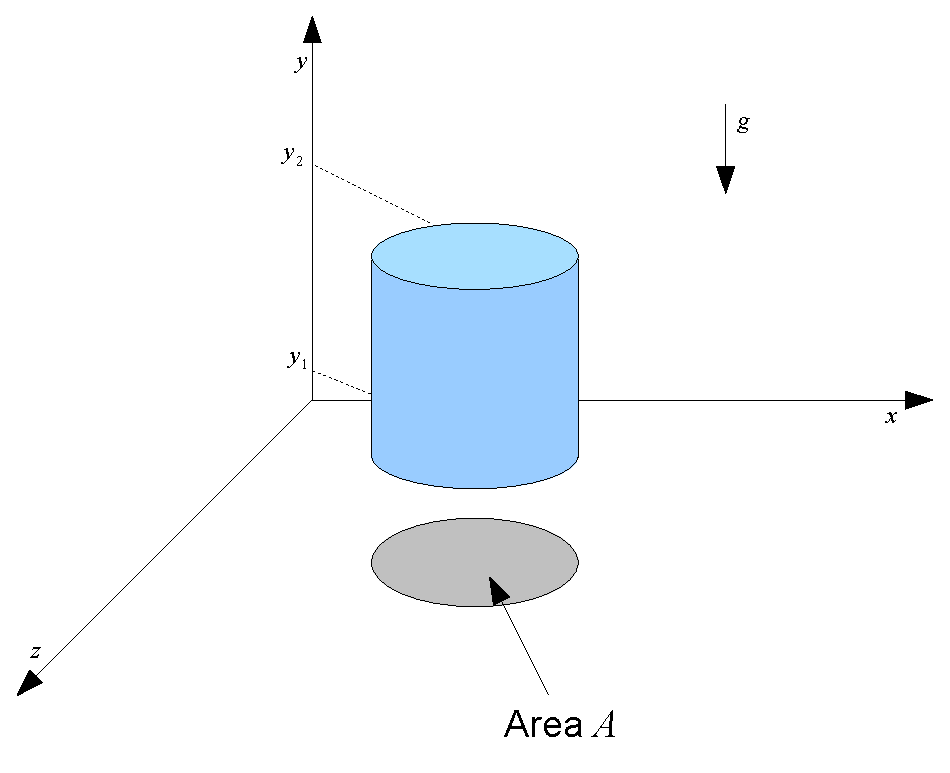
\includegraphics[width=0.7\textwidth]{xyz_cylinder}
\end{center}
Force equilibrium in the $y$ direction in this cylinder requires balance of weight of water column and pressure differential between bottom face $y=y_1$ and top face $y=y_2$.
}

\frame{
Weight of water column:
\[
\mathop{\int\!\!\!\int}_A\int\limits_{y_1}^{y_2}(-\rho g)\ dydxdz
\]
Pressure differential:
\[
\mathop{\int\!\!\!\int}_A\left(p(x,y_2,t)-p(x,y_1,t)\right)\ dxdz
\]
So we must have
\[
\mathop{\int\!\!\!\int}_A\int\limits_{y_1}^{y_2}(-\rho g)\ dydxdz = \mathop{\int\!\!\!\int}_A\left(p(x,y_2,t)-p(x,y_1,t)\right)\ dxdz
\]
}

\frame{
\[
\mathop{\int\!\!\!\int}_A\int\limits_{y_1}^{y_2}(-\rho g)\ dydxdz = \mathop{\int\!\!\!\int}_A\left(p(x,y_2,t)-p(x,y_1,t)\right)\ dxdz
\]
is equivalent to
\[
\mathop{\int\!\!\!\int}_A\int\limits_{y_1}^{y_2}\left(\frac{\partial p}{\partial y}+\rho g\right)\ dydxdz=0
\]
This must be true for any water column, i.e., any $A,y_1,y_2$. Therefore,
\[
\frac{\partial p}{\partial y}+\rho g=0
\]
(otherwise, we would be able to find a water column where the integrand is positive, leading to a positive value of the integral on that column).
}


\frame{\frametitle{Water is incompressible}
If you force a body of water to deform, the volume of that body of water remains constant, i.e., water is an \emph{incompressible fluid}.
\vskip0.5cm
\noindent
$\Rightarrow$ $\rho$, the density, is a constant, and from
\[
\frac{\partial p}{\partial y}+\rho g=0
\]
we get
\[
p=-\rho g y+C,
\]
so if $p$ is measured relative to the pressure above the free upper surface $y=\eta$,
\[
p=\rho g(\eta-y)
\]
}


\frame{\frametitle{Water accumulation}
Consider a fixed volume $V$,
\[
V=\{z_1\leq z\leq z_2,x_1\leq x\leq x_2,-H\leq y\leq\eta\}
\]
\begin{center}
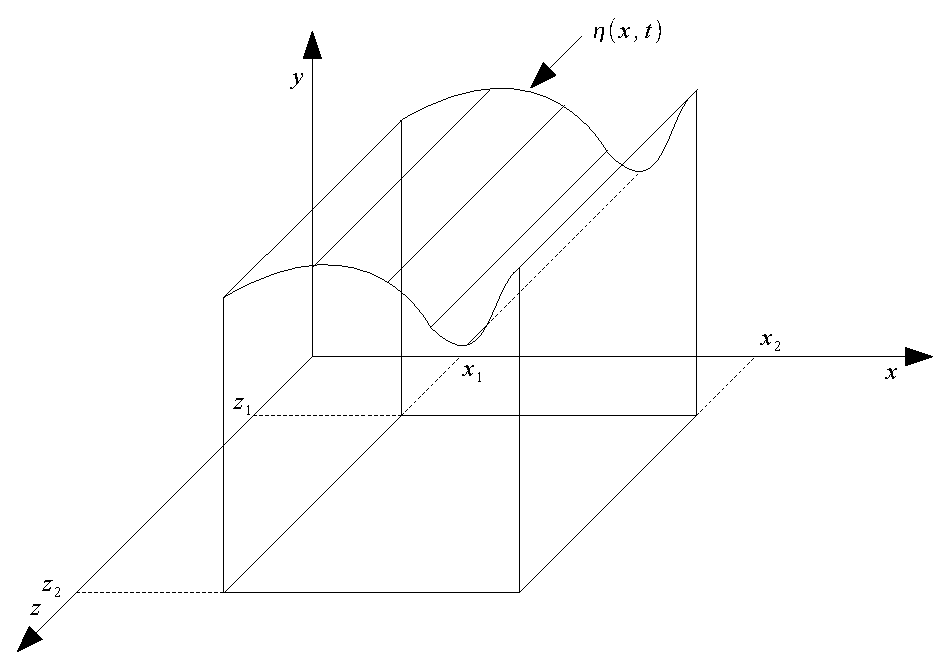
\includegraphics[width=0.7\textwidth]{V_domain}
\end{center}
}

\frame{
Water enters $V$ through $x_1$ face and leaves $V$ through $x_2$ face. 
\begin{center}
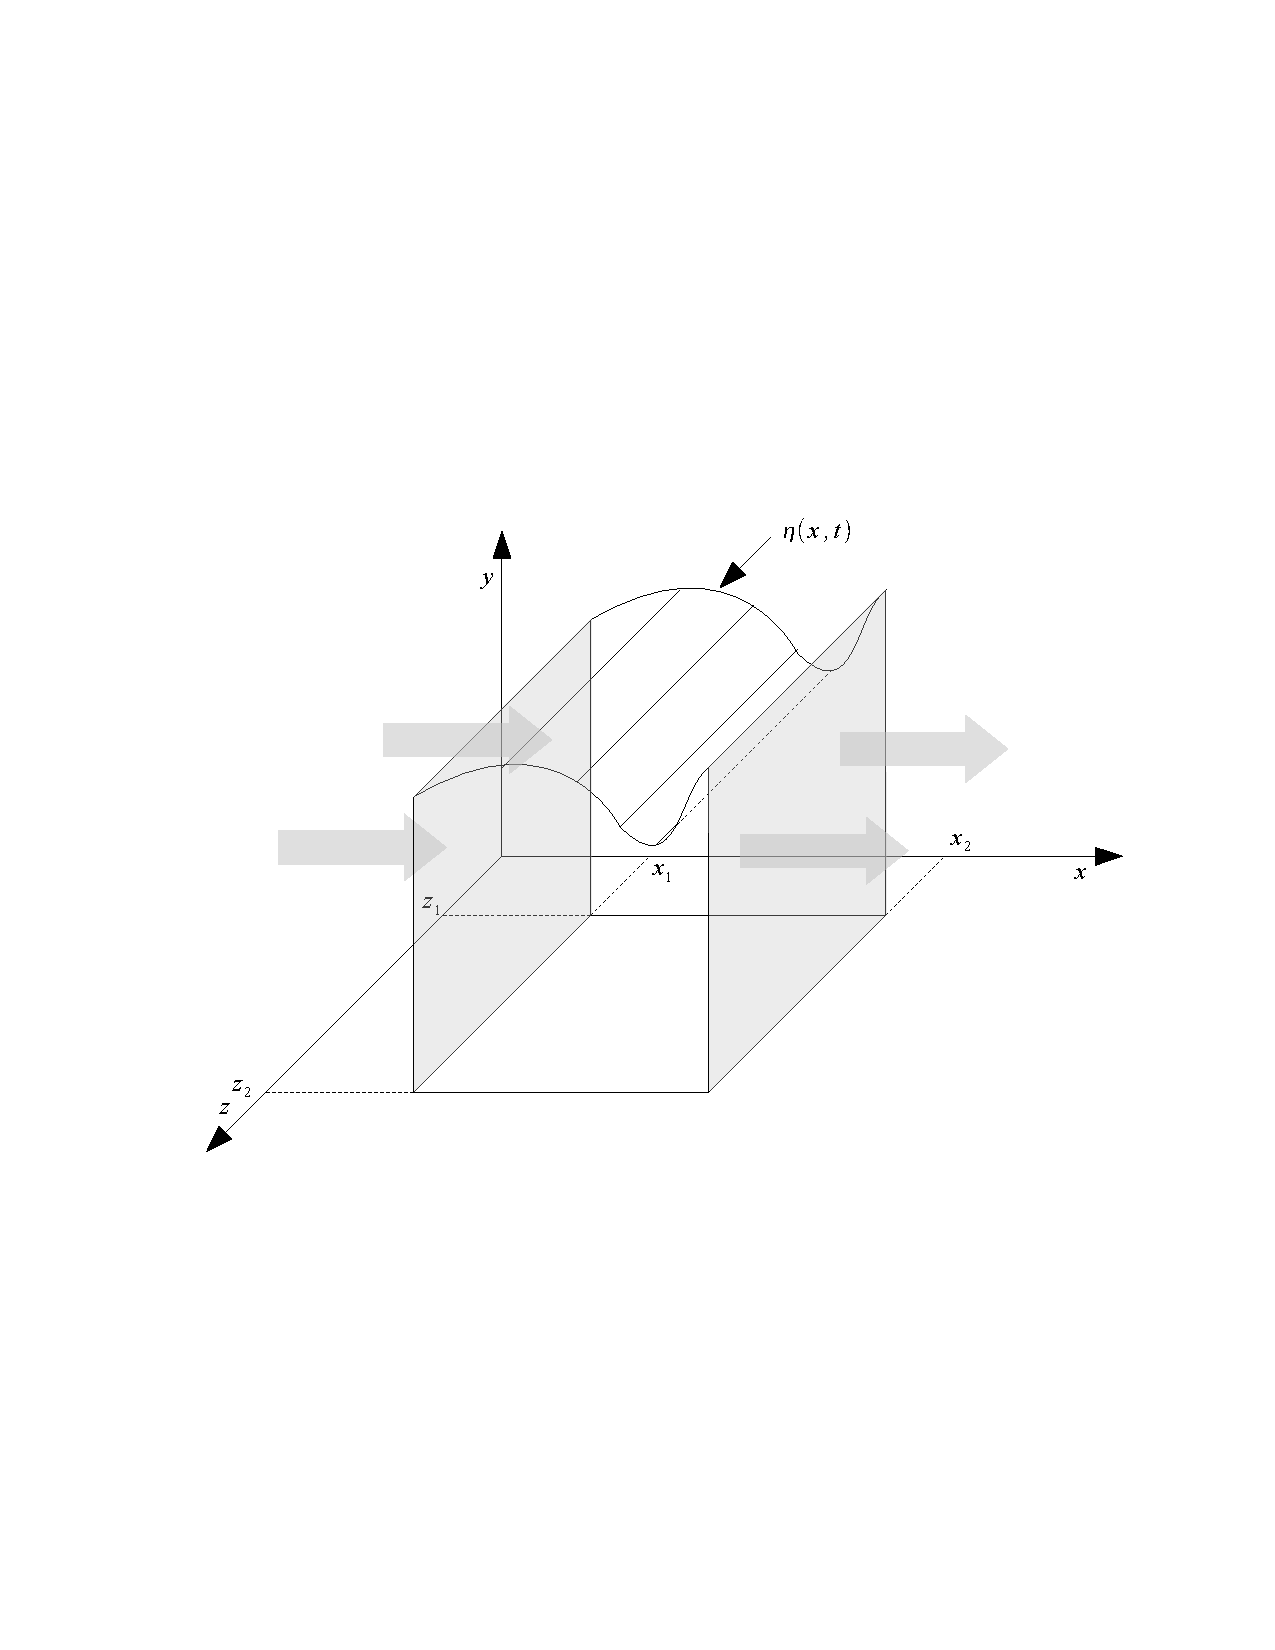
\includegraphics[width=0.7\textwidth]{V_domain_flows}
\end{center}
Rate of water accumulation in $V$ is
\[
\frac{d}{dt}\int_{z_1}^{z_2}\int_{x_1}^{x_2}\int_{-H}^\eta \rho\ dydxdz =\Delta z\frac{d}{dt}\int_{x_1}^{x_2}\rho h\ dx,
\]
with $\Delta z=z_2-z_1$, and $h(x,t)=\eta+H$ the height of water at time $t$ at spatial location $x$.
}

\frame{\frametitle{Water flux}
Net flux of water entering $V$ through its faces $x=x_1$ and $x=x_2$ is
\begin{center}
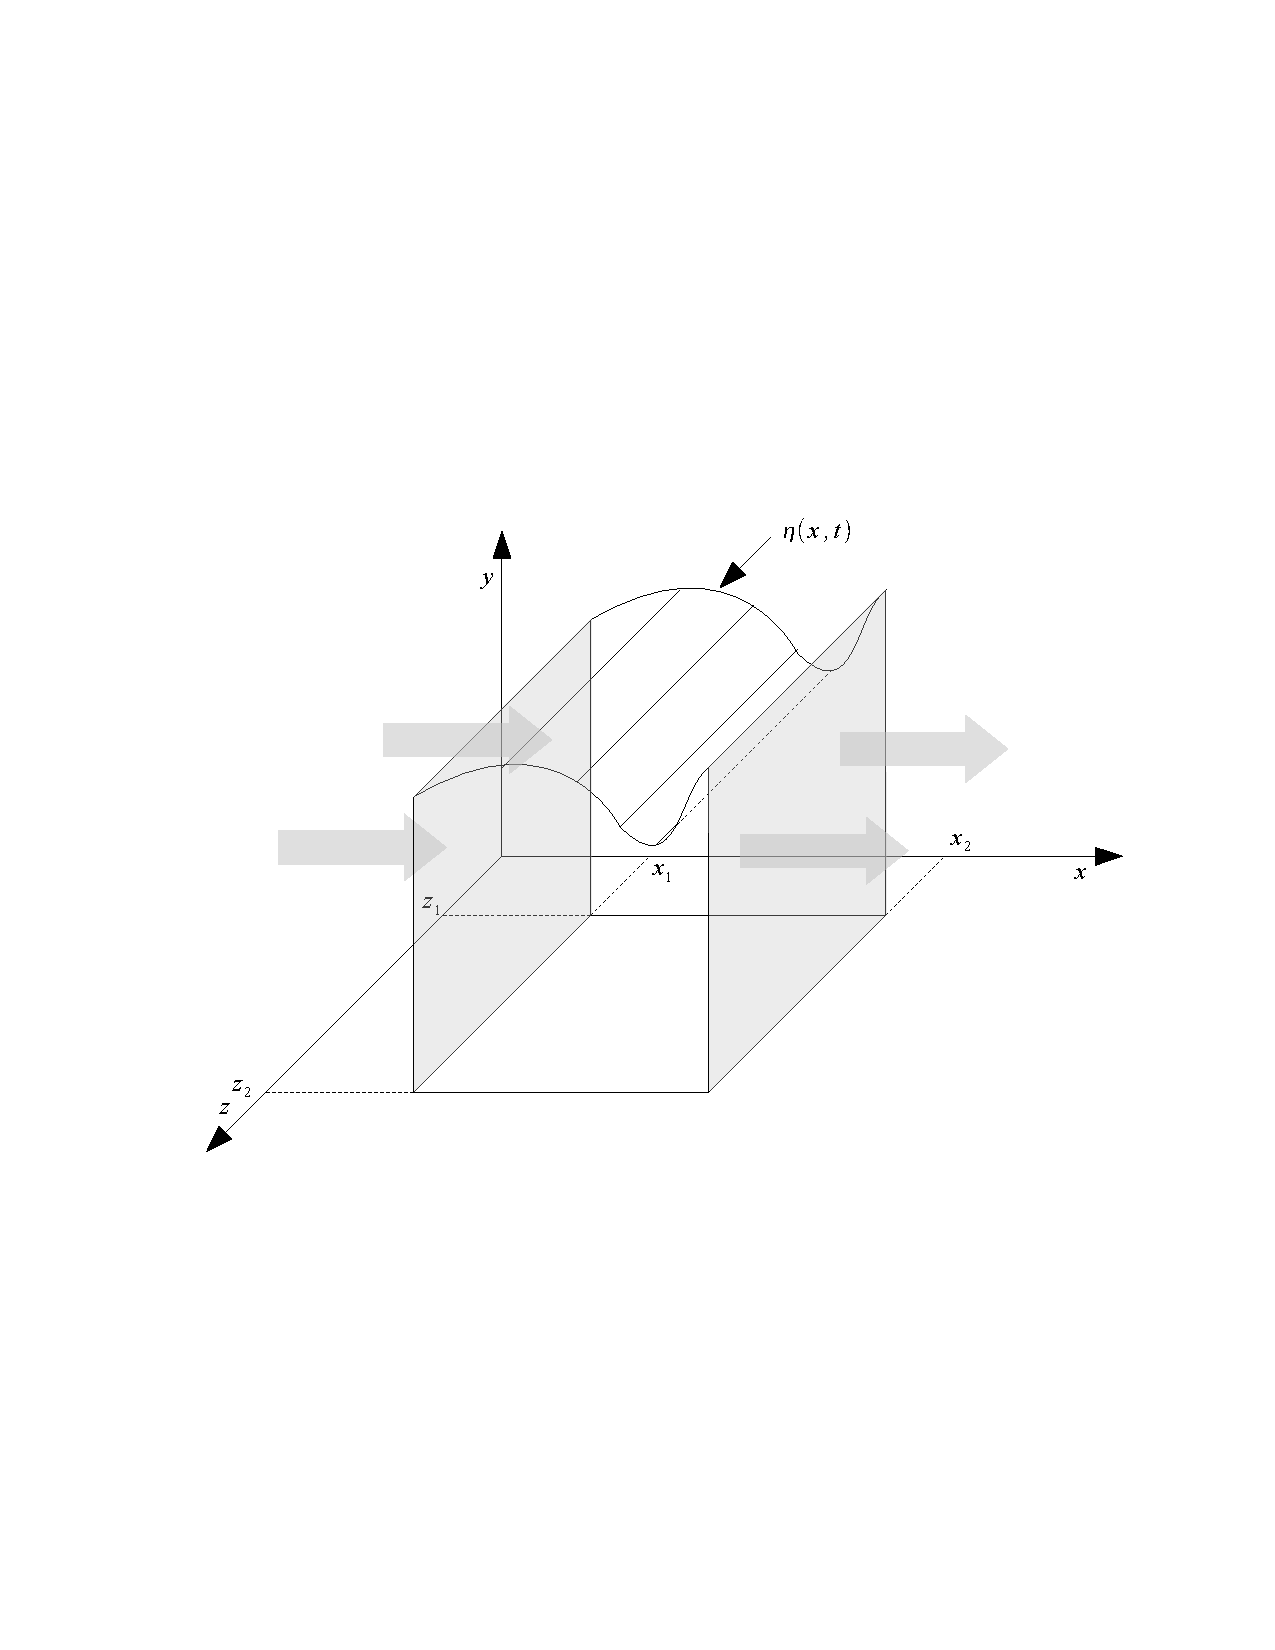
\includegraphics[width=0.7\textwidth]{V_domain_flows}
\end{center}
\[
\left[\int_{z_1}^{z_2}\int_{-H}^\eta u\ dydz\right]_{x=x_1}
-\left[\int_{z_1}^{z_2}\int_{-H}^\eta u\ dydz\right]_{x=x_2} 
=-\Delta z\left[\rho uh\right]_{x_1}^{x_2}
\]
There is no flux through $y=-H$ and $y=\eta$, and no net flux through $z=z_1$ and $z=z_2$.
}

\frame{\frametitle{Conservation of mass}
Of course, the mass must conserve in $V$, so the two expressions must be equal, i.e.,
\[
\frac{d}{dt}\int\limits_{x_1}^{x_2} \rho h\ dx+\left[\rho uh\right]_{x_1}^{x_2}=0
\]
}

\frame{
Newton's second law for deformable media (Euler): rate of increase of horizontal momentum (in the $x$ direction) in $V$ must equal the sum of the net influx of momentum into the volume and the net horizontal force acting on the column.
\vskip0.2cm
(Momentum: product of mass and velocity of an object).
\vskip0.5cm
Rate of increase of momentum
\[
\frac{d}{dt}\int\limits_{z_1}^{z_2}\int\limits_{x_1}^{x_2}\int\limits_{-H}^\eta \rho u\ dydxdz
=\Delta z\frac{d}{dt}\int\limits_{x_1}^{x_2}\rho uh dx
\]
}

\frame{\frametitle{Momentum flux}
Net influx of momentum through faces $x=x_1$ and $x=x_2$ is
\begin{multline*}
\left[\int\limits_{z_1}^{z_2}\int\limits_{-H}^\eta (\rho u)u\ dydz\right]_{x=x_1}
-\left[\int\limits_{z_1}^{z_2}\int\limits_{-H}^\eta (\rho u)u\ dydz\right]_{x=x_2} \\
=-\Delta z\left[\rho u^2h\right]_{x_1}^{x_2}
\end{multline*}
There is no flux through $y=-H$ and $y=\eta$, and no net flux through $z=z_1$ and $z=z_2$.
}

\frame{\frametitle{Forces acting on $V$}
Ignore friction at $y=-H$. Then only contributions to horizontal forces come from pressure at $x=x_1$ and $x=x_2$, so net horizontal forces acting on $V$ is
\begin{align*}
\left[\int\limits_{z_1}^{z_2}\int\limits_{-H}^\eta p\ dydz\right]_{x_1}^{x_2} &=
-\left[\Delta z\int\limits_{-H}^\eta \rho g(\eta-y)\ dy\right]_{x_1}^{x_2} \\
&= \left[\left.-\Delta z\rho g(\eta y-\frac 12 y^2)\right|_{-H}^\eta\right]_{x_1}^{x_2} \\
&=\left[-\frac 12 \Delta z\rho g h^2\right]_{x_1}^{x_2}
\end{align*}
}

\frame{\frametitle{Conclusion from Newton's second law}
\[
\frac{d}{dt}\int\limits_{x_1}^{x_2}\rho uh\ dx
+\left[\rho u^2h+\frac 12\rho gh^2\right]_{x_1}^{x_2}=0
\]
}

\frame{\frametitle{The general model}
Pressure magnitude:
\begin{equation}\label{eq:pressure}
p=\rho g(\eta-y)
\end{equation}
Horizontal velocity:
\begin{equation}\label{eq:horiz_velocity}
\frac{d}{dt}\int\limits_{x_1}^{x_2} \rho h\ dx+\left[\rho uh\right]_{x_1}^{x_2}=0
\end{equation}
Free surface height:
\begin{equation}\label{eq:free_surf}
\frac{d}{dt}\int\limits_{x_1}^{x_2}\rho uh\ dx
+\left[\rho u^2h+\frac 12\rho gh^2\right]_{x_1}^{x_2}=0
\end{equation}
}


\section{Case of smooth solutions}
\frame[plain]{\tableofcontents[current]}


\frame{
Suppose $u$ and $h$ are smooth (with continuous first order partial derivatives),
then \eqref{eq:horiz_velocity} and \eqref{eq:free_surf} take a much simpler form,
\[
\int_{x_1}^{x_2}\left(\frac{\partial h}{\partial t}+\frac{\partial}{\partial x}(uh)\right)\ dx=0
\]
and
\[
\int_{x_1}^{x_2}\left(\frac{\partial}{\partial t}(uh)+\frac{\partial}{\partial x}(u^2h+\frac 	12gh^2)\right)\ dx=0
\]
Since the intervals of integration $[x_1,x_2]$ are arbitrary, and that the integrands are continuous, we have
\[
\frac{\partial h}{\partial t}+\frac{\partial}{\partial x}(uh)=0
\]
and
\[
\frac{\partial}{\partial t}(uh)+\frac{\partial}{\partial x}(u^2h+\frac 	12gh^2)=0
\]
}

\frame{
We write
\[
\frac{\partial h}{\partial t}+\frac{\partial}{\partial x}(uh)=0
\]
and
\[
\frac{\partial}{\partial t}(uh)+\frac{\partial}{\partial x}(u^2h+\frac 	12gh^2)=0
\]
as
\begin{align}
h_t+(uh)_x&=0 \label{eq:h2}\\
\intertext{and}
(uh)_t+(u^2h+\frac 12gh^2)_x &=0 \label{eq:u2}
\end{align}
}

\frame{
From \eqref{eq:h2},
\[
h_t=-(uh)_x=-(u_xh+uh_x)
\]
Equation \eqref{eq:u2} can be rewritten as
\begin{align*}
\eqref{eq:u2} &\Leftrightarrow u_th+uh_t+(u^2h+\frac 12gh^2)_x=0 \\
&\Leftrightarrow 
u_th-u(u_xh+uh_x)+2uu_xh+u^2h_x+ghh_x=0 \\
&\Leftrightarrow u_th-uu_xh-\cancel{u^2h_x}+2uu_xh+\cancel{u^2h_x}+ghh_x=0 \\
&\Leftrightarrow u_th+uu_xh+ghh_x=0
\end{align*}
Therefore, provided $h\neq 0$, we get
\begin{subequations}\label{sys:smooth}
\begin{align}
h_t+(uh)_x&=0 \label{eq:h}\\
u_t+uu_x+gh_x &=0 \label{eq:u}
\end{align}
\end{subequations}
which describes the evolution of $u$ and $h$. 
}

\frame{\frametitle{The model for smooth solutions}
\begin{align}
h_t+(uh)_x&=0 \tag{\ref{eq:h}}\\
u_t+uu_x+gh_x &=0 \tag{\ref{eq:u}}
\end{align}
If $-\infty<x<\infty$, then all we need is an initial condition, i.e., functions describing the initial state of $u$ and $h$:
\[
u(x,0)=u_0(x),\quad h(x,0)=h_0(x), \qquad -\infty<x<\infty.
\]
If $x$ has a boundary, then we need boundary conditions.
}

\section{Linearization}
\frame[plain]{\tableofcontents[current]}


\frame{
Suppose the bottom is flat ($H$ is constant), and that the deviation from the undisturbed depth $H$ is small compared to $H$ itself, then
\[
h=(H+\zeta)=H(1+\frac \zeta H)\simeq H,\qquad h_t=\zeta_t,\qquad h_x=\zeta_x.
\]
If $|u|$ is also small, then $uu_x$ can be neglected. Then we can linearize
\begin{align}
h_t+(uh)_x&=0 \tag{\ref{eq:h}}\\
u_t+uu_x+gh_x &=0, \tag{\ref{eq:u}}
\end{align}
getting
\begin{subequations}\label{sys:small_amp}
\begin{align}
\zeta_t+Hu_x &= 0 \label{eq:zeta_t} \\
u_t+g\zeta_x &= 0 \label{eq:zeta_x}
\end{align}
\end{subequations}
}

\frame{
Differentiate \eqref{eq:zeta_x} with respect to $x$:
\[
u_{tx}+g\zeta_{xx}=0
\]
and therefore,
\begin{equation}\label{eq:u_tx}
u_{tx}=-g\zeta_{xx}
\end{equation}
Differentiate \eqref{eq:zeta_t} with respect to $t$:
\begin{equation}\label{eq:zeta_tt}
\zeta_{tt}+Hu_{xt}=0
\end{equation}
If $u$ has continuous second-order partial derivatives, then from Clairaut's theorem, $u_{tx}=u_{xt}$. Therefore, substituting \eqref{eq:u_tx} into \eqref{eq:zeta_tt},
\[
\zeta_{tt}-HG\zeta_{xx}=0
\]
that is
\[
\zeta_{tt}=c^2\zeta_{xx}, \qquad c^2=Hg
\]
}


\frame{\frametitle{The one-dimensional wave equation (1)}
The partial differential equation
\begin{equation}\label{eq:wave_zeta}
\zeta_{tt}=c^2\zeta_{xx}
\end{equation}
with $c^2=Hg$, is the one-dimensional wave equation. Initial conditions are given by
\begin{align*}
\zeta(x,0) &= h_0(x)-H\equiv\zeta_0(x) \\
\zeta_t(x,0) &= -Hu_x(x,0)=-H[u_0(x)]_x\equiv \nu_0(x)
\end{align*}
}

\frame{\frametitle{The one-dimensional wave equation (2)}
Things can also be expressed in terms of $u$. Using the same type of simplification used before for $\zeta$, we get
\begin{equation}\label{eq:wave_u}
u_{tt}=c^2u_{xx}
\end{equation}
with $c^2=Hg$. Initial conditions are given by
\begin{align*}
u(x,0) &= u_0(x) \\
u_t(x,0) &= -g\zeta_x(x,0)=-g[h_0(x)]_x\equiv v_0(x)
\end{align*}
}

\section{Traveling wave solutions}
\frame[plain]{\tableofcontents[current]}


\frame{\frametitle{Traveling wave solutions}
This was obtained by d'Alembert. Consider
\begin{equation}
u_{tt}=c^2u_{xx} \tag{\ref{eq:wave_u}}
\end{equation}
Note that this can be written as
\[
\left(\frac{\partial}{\partial t}-c\frac{\partial}{\partial x}\right)
\left(\frac{\partial}{\partial t}+c\frac{\partial}{\partial x}\right)u=0
\]
This implies that for any $F,G$, the sum
\[
u(x,t)=F(x-ct)+G(x+ct)
\]
satisfies \eqref{eq:wave_u}.
}

\frame{\frametitle{Derivation of the solution}
Introduce the new variables
\[
a=x-ct\qquad\textrm{and}\qquad b=x+ct
\]
We have
\[
\frac{\partial u}{\partial x}=\frac{\partial u}{\partial a}+\frac{\partial u}{\partial b}\qquad
\frac{\partial u}{\partial t}=-c\frac{\partial u}{\partial a}+c\frac{\partial u}{\partial b}
\]
\[
\frac{\partial^2}{\partial x^2}u=\left(\frac{\partial}{\partial a}+\frac{\partial}{\partial b}\right)^2 u=\frac{\partial^2u}{\partial a^2}+2\frac{\partial^2u}{\partial a\partial b}+\frac{\partial^2u}{\partial b^2}
\]
\[
\frac{\partial^2}{\partial t^2}u=\left(-c\frac{\partial}{\partial a}+c\frac{\partial}{\partial b}\right)^2u=c^2\left(\frac{\partial^2u}{\partial a^2}-2\frac{\partial^2u}{\partial a\partial b}+\frac{\partial^2u}{\partial b^2}\right)
\]
}

\frame{
So the equation
\begin{equation}
u_{tt}=c^2u_{xx} \tag{\ref{eq:wave_u}}
\end{equation}
is written
\[
4\frac{\partial^2 u}{\partial a\partial b}=0
\]
Integrate with respect to b:
\[
\frac{\partial u}{\partial a}=\xi(a)
\]
and thus
\begin{align*}
u(x,t)=u(a,b) &= \int \xi(a)da+G(b)\\
&=F(a)+G(b)\\
&=F(x-ct)+G(x+ct)
\end{align*}
}

\frame{
Set
\[
u(x,0)=f(x)\qquad u_t(x,0)=g(x)
\]
Then d'Alembert's formula gives
\[
u(x,t) = \frac{f(x-ct) + f(x+ct)}{2} + \frac{1}{2c} \int_{x-ct}^{x+ct} g(s) ds
\]
}

\frame{\frametitle{Case of a Dirac delta initial condition}
Suppose $u_0(x)=0$ and $v_0(x)=\delta(x)$, for $-\infty<x<\infty$, with $\delta$ the Dirac delta,
\[
\delta(x)=\begin{cases}
\infty & \textrm{if }x=0\\
0 & \textrm{otherwise}.
\end{cases}
\]
Therefore,
\[
u(x,t)=\frac 1{2c}\int_{x-ct}^{x+ct}\delta(z)dz=\frac 1{2c}\left\{H(x+ct)-H(x-ct)\right\},
\]
with $H$ the Heaviside function,
\[
H(x)=\begin{cases}
0 & \textrm{if }x<0\\
1 & \textrm{if }x>0.
\end{cases}
\]
}

\frame{
For simplicity, take $c=1$. This gives
\[
u(x,t)=\frac 12\left\{H(x+t)-H(x-t)\right\},
\]
}

\frame{
\begin{center}
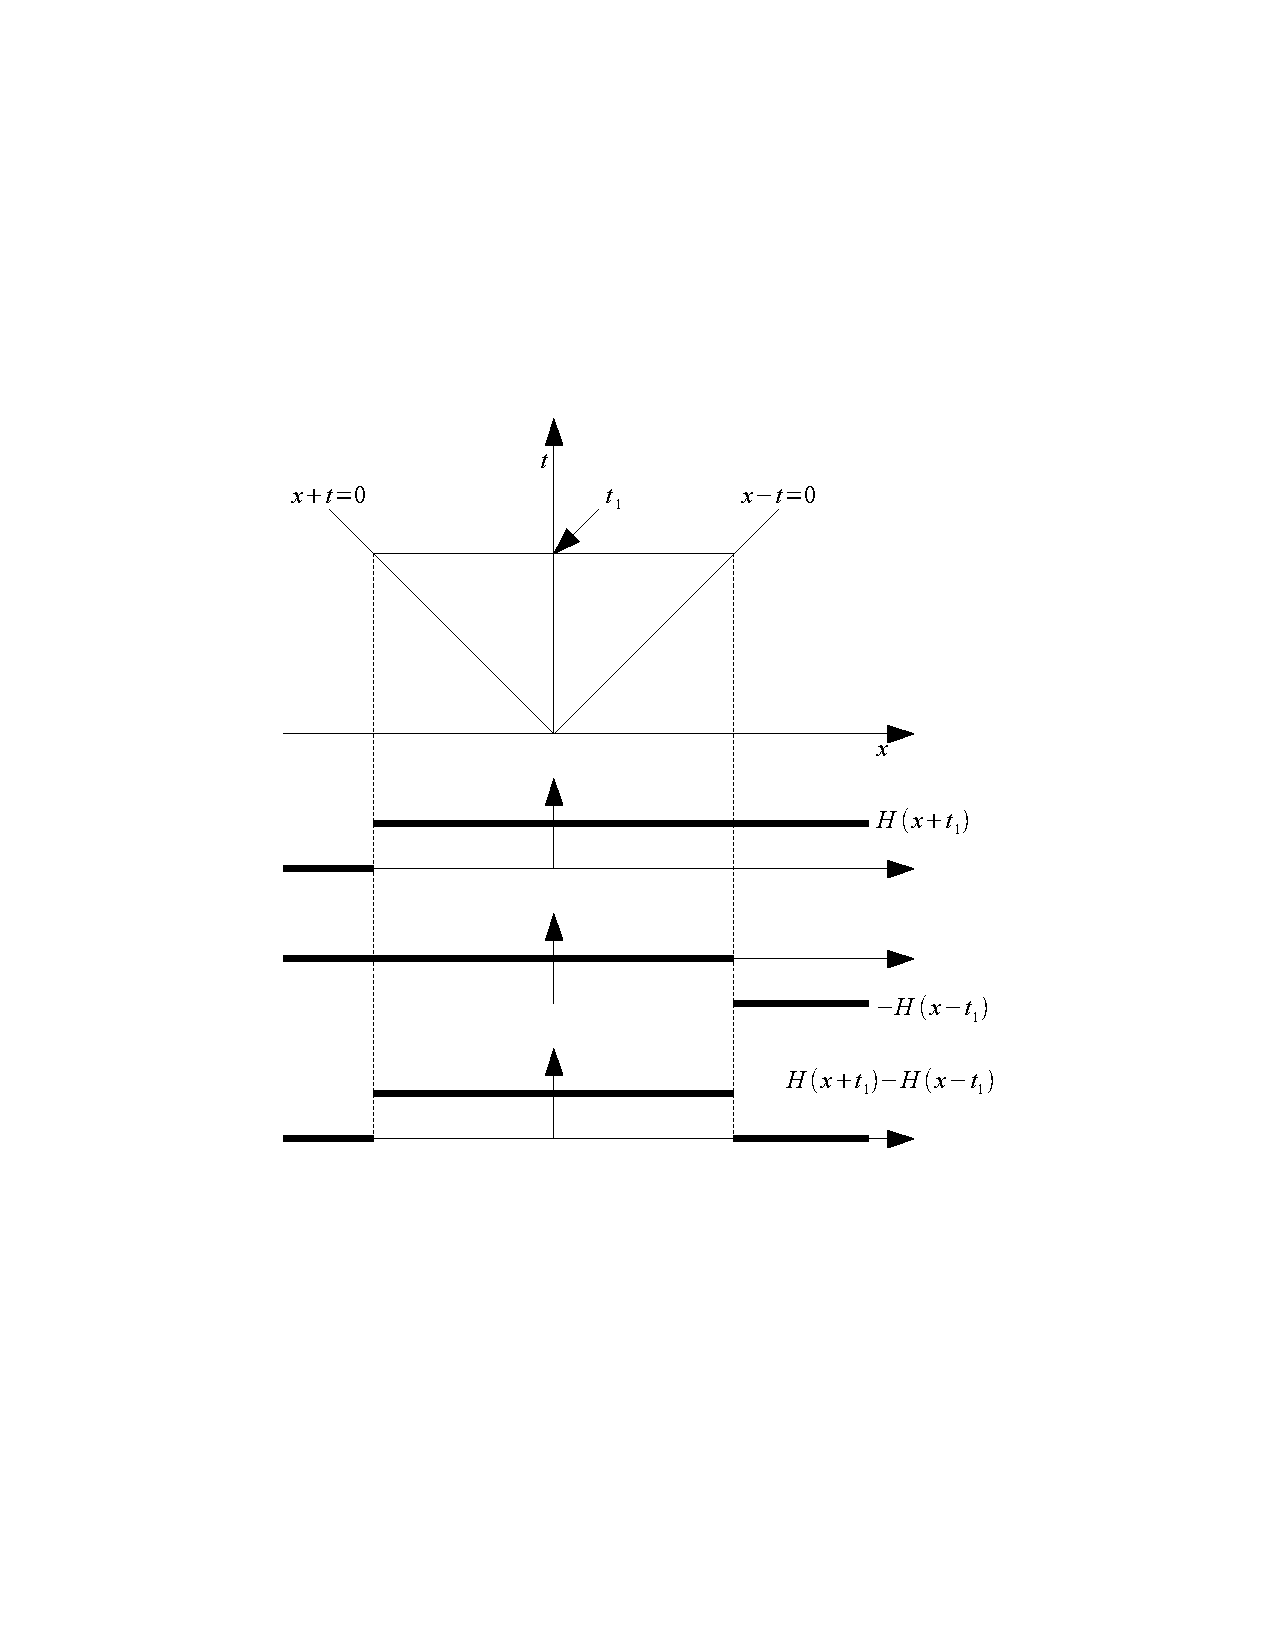
\includegraphics[height=0.95\textheight]{xct}
\end{center}
}

\frame{
As $t$ increases, we move further up in the top graph in $(x,t)$-space, resulting in a wider and wider square pulse.
\begin{center}
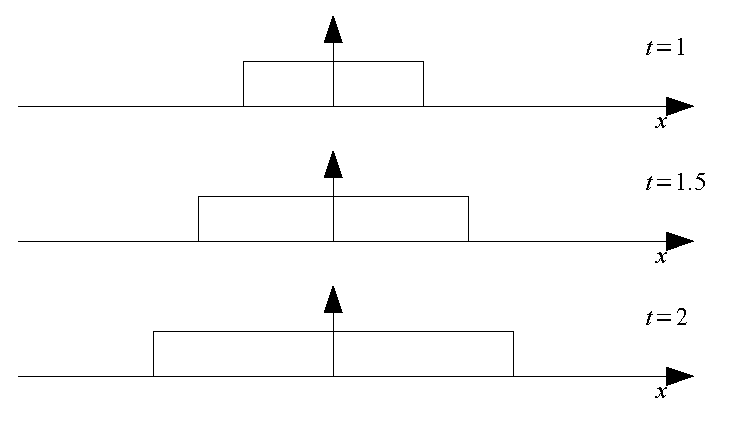
\includegraphics[width=\textwidth]{xwave}
\end{center}
}

\end{document}